\documentclass[12pt]{article}

% Layout.
\usepackage[top=1in, bottom=0.75in, left=1in, right=1in, headheight=1in, headsep=6pt]{geometry}

% Fonts.
\usepackage{mathptmx}
\usepackage[scaled=0.86]{helvet}
\renewcommand{\emph}[1]{\textsf{\textbf{#1}}}

% TiKZ.
\usepackage{tikz, pgfplots}

\usetikzlibrary{calc,trees,positioning,arrows,fit,shapes,through, backgrounds}
\usetikzlibrary{patterns}

\usetikzlibrary{decorations.markings}
\usetikzlibrary{arrows}

\usepackage{pgfplots}


% Misc packages.
\usepackage{amsmath,amssymb,latexsym}
\usepackage{graphicx}
\usepackage{array}
\usepackage{xcolor}
\usepackage{multicol}
\usepackage{fancyhdr}
\pagestyle{fancy}


% Misc.
\renewcommand{\d}{\displaystyle}
\newcommand{\ds}{\displaystyle}
\newcommand{\ul}[1]{\underline{#1}}
\def\bc{\begin{center}}
\def\ec{\end{center}}
\def\be{\begin{enumerate}}
\def\ee{\end{enumerate}}

\newcommand{\ans}[1][1in]{\rule{#1}{.5pt}}


\lhead{Math F113X: Quiz 5}
\rhead{Date: \hspace{2cm}}

\begin{document}

\vspace{1cm}
\strut

\noindent \textbf{Name:} \hrulefill \quad  score:\ans[1cm] \ / 10 \\


\noindent There are 10 points possible on this quiz. No aids (book, notes, etc.)
are permitted. You may use a calculator.  {\bf Show all work and supporting calculations for full credit. Explain how you get your answers.}



\be

\item (3 points) Consider the following graph.

\be
\item There is an Euler path in this graph. Without explicitly finding the path, what must the starting and stopping vertices be, and how do you know those are the starting and stopping vertices?

\hfill 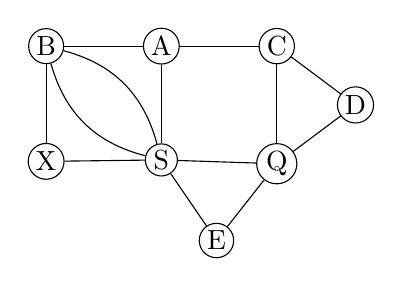
\begin{tikzpicture}[vtx/.style={draw, circle, inner sep = 1 pt}]
\node[vtx] (A) {A};
\node[vtx,left = of A] (B) {B};
\node[vtx,right = of A] (C) {C};
\node[vtx, below = of C] (Q) {Q};
\node[vtx] (D) at ($(C)!0.5!(Q)!1cm!90:(Q)$) {D};
\node[vtx, below = of A] (S) {S};
\node[vtx, below = of B](X) {X};
\node[vtx] (E) at ($(S)!0.5!(Q)!1cm!90:(S)$) {E};
\foreach \i/\j in {A/B, A/C, B/X, S/X, S/Q, C/Q, C/D, Q/D, A/S, S/E, E/Q} {\draw (\i) -- (\j);}
%\draw (B) to[out = 180+45, in = 180 + 45, distance = 2cm] (S);
\draw (B) to[bend left = 30] (S);
\draw (B) to[bend right = 30] (S);
\end{tikzpicture}

\item \emph{Draw} the Euler path on the graph in one continuous path offset slightly from your graph, with arrows showing the direction of travel. Also \emph{list} the vertices in your path in the order you encounter them.

\bigskip

Path \hrulefill

\ee

\item (3 points) Given the graph below, use Kruskal's algorithm to find a minimum cost spanning tree. The edges in sorted order have been provided to you. Draw the minimum cost spanning tree on the blank copy of the graph, and indicate for each edge in the chart whether you are using it or not.

%\begin{tikzpicture}[vtx/.style={draw, circle, inner sep = 1 pt}, lbl/.style={font = \scriptsize, inner sep = 1 pt, fill = white}]
%\node[vtx] (A) at (0:2){A};
%\node[vtx] (B) at (360/6:2) {B};
%\node[vtx] (C) at (360*2/6:2) {C};
%\node[vtx] (D) at (360*3/6:2) {D};
%\node[vtx] (E) at (360*4/6:2) {E};
%\node[vtx] (F) at (360*5/6:2) {F};
%\foreach \i/\j/\k in {A/B/5, %A/C/6,
%A/E/5,A/F/4,B/C/1,B/D/2,B/E/11,B/F/18,C/E/15,C/D/2,D/E/10,E/F/1}{
%\draw (\i) -- node[midway,lbl]{\k} (\j);}
%\draw (A) -- node[lbl, pos = .6]{6} (C);
%\end{tikzpicture}


\tikzset{vtx/.style={draw, circle, inner sep=1pt},
         lbl/.style={font=\scriptsize, inner sep=1pt, fill=white}}
         
\newcommand{\gvertices}{%
  \node[vtx] (A) at (0:2) {A};
  \node[vtx] (B) at (360/6:2) {B};
  \node[vtx] (C) at (360*2/6:2) {C};
  \node[vtx] (D) at (360*3/6:2) {D};
  \node[vtx] (E) at (360*4/6:2) {E};
  \node[vtx] (F) at (360*5/6:2) {F};
}

%
%---------------------------------------------- (1) the graph
\begin{minipage}[t]{0.35\textwidth}
\vspace{0pt}\centering
\begin{tikzpicture}[baseline=(current bounding box.north)]
  \gvertices
  \foreach \i/\j/\k in {A/B/11, A/E/11, A/F/4, B/C/2, B/D/2, B/E/3, B/F/8,
                        C/E/4, C/D/3, D/E/4, E/F/14}{
    \draw (\i) -- node[midway,lbl]{\k} (\j);}
  \draw (A) -- node[lbl, pos=.6]{9} (C);
\end{tikzpicture}
\end{minipage}%
%---------------------------------------------- (2) the chart
\begin{minipage}[t]{0.28\textwidth}
\vspace{0pt}\centering
\renewcommand{\arraystretch}{1}
\begin{tabular}{|c|c|c|}
\hline
\textbf{edge} & \textbf{weight} & \textbf{used} \\ \hline
$BC$ & 2 & \\ \hline
$BD$ & 2 & \\ \hline
$BE$ & 3 & \\ \hline
$CD$ & 3 & \\ \hline
$AF$ & 4 & \\ \hline
$CE$ & 4 & \\ \hline
$DE$ & 4 & \\ \hline
$BF$ & 8 & \\ \hline
$AC$ & 9 & \\ \hline
$AB$ & 11 & \\ \hline
$AE$ & 11 & \\ \hline
$EF$ & 14 & \\ \hline
\end{tabular}
\end{minipage}%
%
%---------------------------------------------- (3) blank copy
\begin{minipage}[t]{0.35\textwidth}
\vspace{0pt}\centering
\begin{tikzpicture}[baseline=(current bounding box.north),vtx/.style={draw, circle, inner sep = 1 pt}, lbl/.style={font = \scriptsize, inner sep = 1 pt, fill = white}]
  \gvertices
\end{tikzpicture}
\end{minipage}

\bigskip

 What is the total weight of the spanning tree? \ans

\newpage

\item In a certain city there is a river running through the middle of the city. There are three islands and ten bridges, as shown in the figure. A tourist wants to start at their hotel on the north bank, stroll across every bridge at least once, and return to their hotel at the end of their trip.

\be
\item {(2 points)} Make a graph model of this scenario. (This means make a graph that represents the situation.) Label the vertices appropriately.

\bigskip

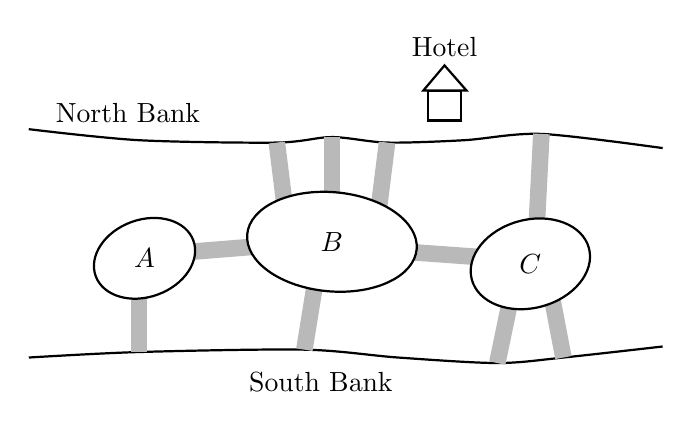
\begin{tikzpicture}[
  bridge/.style={line width=6pt, gray!55},
  blob/.style={draw, thick, fill=white},
  bank/.style={thick}
]
% ---- landing points on the banks (the curves pass exactly through these) ----
\coordinate (N1) at (2.80,2.80);
\coordinate (N2) at (3.50,2.87);
\coordinate (N3) at (4.20,2.80);
\coordinate (N4) at (6.16,2.91);
\coordinate (S1) at (1.05,0.14);
\coordinate (S2) at (5.60,0.00);
\coordinate (S3) at (6.44,0.07);
\coordinate (S4) at (3.15,0.17);

% ---- banks ----
\draw[bank] plot[smooth] coordinates {(-0.35,2.97) (1.05,2.83) (N1) (N2) (N3) (5.18,2.83) (N4) (7.70,2.73)};
\draw[bank] plot[smooth] coordinates {(-0.35,0.07) (S1) (S4) (4.34,0.07) (S2) (S3) (7.70,0.21)};
\node[font=\normalsize] at (0.91,3.18) {North Bank};
\node[font=\normalsize] at (3.36,-0.24) {South Bank};

% ---- bridges (drawn first so the islands sit on top of their ends) ----
% three from B to the North Bank
\draw[bridge] (2.94,1.68) -- (N1);
\draw[bridge] (3.50,1.82) -- (N2);
\draw[bridge] (4.06,1.68) -- (N3);
% one from C to the North Bank
\draw[bridge] (6.09,1.54) -- (N4);
% A -- B, B -- C
\draw[bridge] (1.54,1.40) -- (2.80,1.50);
\draw[bridge] (4.20,1.43) -- (5.60,1.33);
% A to the South Bank
\draw[bridge] (1.05,1.05) -- (S1);
% one from B to the South Bank
\draw[bridge] (3.32,1.22) -- (S4);
% two from C to the South Bank
\draw[bridge] (5.81,1.01) -- (S2);
\draw[bridge] (6.26,1.01) -- (S3);

% ---- islands ----
\draw[blob, rotate around={20:(1.12,1.33)}]  (1.12,1.33) ellipse (0.66 and 0.49);
\draw[blob, rotate around={-5:(3.50,1.54)}]  (3.50,1.54) ellipse (1.08 and 0.63);
\draw[blob, rotate around={15:(6.02,1.26)}]  (6.02,1.26) ellipse (0.77 and 0.56);
\node[font=\normalsize] at (1.12,1.33) {$A$};
\node[font=\normalsize] at (3.50,1.54) {$B$};
\node[font=\normalsize] at (6.02,1.26) {$C$};

% ---- hotel: square with a triangular roof, standing on the North Bank ----
\draw[thick, fill=white] (4.72,3.08) rectangle (5.14,3.46);
\draw[thick, fill=white] (4.66,3.46) -- (4.93,3.78) -- (5.21,3.46) -- cycle;
\node[font=\normalsize] at (4.93,4.02) {Hotel};
\end{tikzpicture}

\bigskip

\bigskip

\item (2 points) Suppose there is a \$1.00 toll to cross each bridge. What is the cheapest possible cost of such a trip, and how do you know? (Explain your reasoning.)

\ee

 \ee
\end{document}